\documentclass{article}
\usepackage{pgfplots}
\pgfplotsset{compat=1.18}

\begin{document}

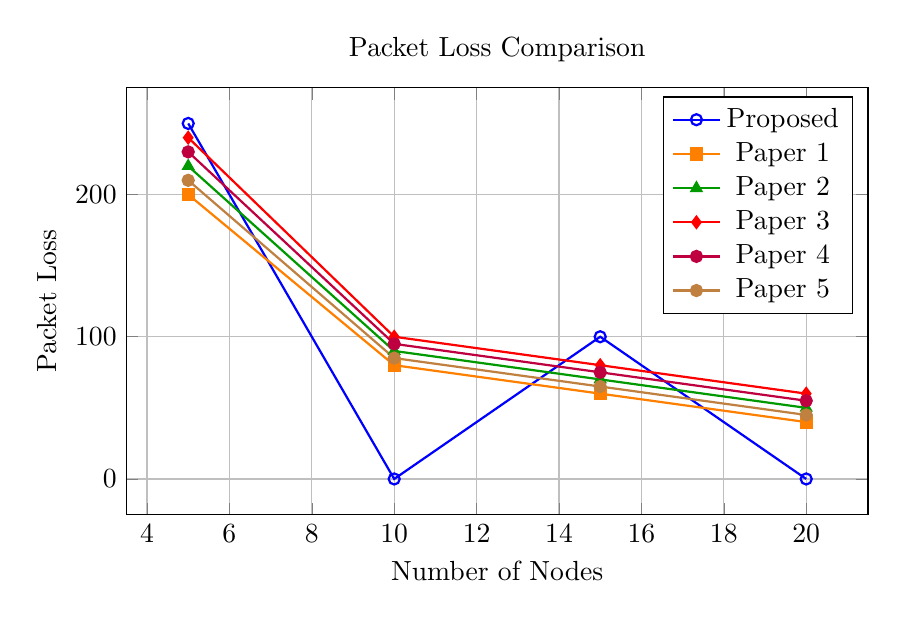
\begin{tikzpicture}
\begin{axis}[
    title={Packet Loss Comparison},
    xlabel={Number of Nodes},
    ylabel={Packet Loss},
    width=11cm,
    height=7cm,
    grid=major,
    legend style={
        at={(0.98,0.98)},   % top-left (no overlap)
        anchor=north east,
        draw=black,
        fill=white
    }
]

% Proposed (NS3)
\addplot[blue, mark=o, thick] coordinates {
    (5,250) (10,0) (15,100) (20,0)
};

% Paper 1
\addplot[orange, mark=square*, thick] coordinates {
    (5,200) (10,80) (15,60) (20,40)
};

% Paper 2
\addplot[green!60!black, mark=triangle*, thick] coordinates {
    (5,220) (10,90) (15,70) (20,50)
};

% Paper 3
\addplot[red, mark=diamond*, thick] coordinates {
    (5,240) (10,100) (15,80) (20,60)
};

% Paper 4
\addplot[purple, mark=*, thick] coordinates {
    (5,230) (10,95) (15,75) (20,55)
};

% Paper 5
\addplot[brown, mark=*, thick] coordinates {
    (5,210) (10,85) (15,65) (20,45)
};

\legend{Proposed , Paper 1, Paper 2, Paper 3, Paper 4, Paper 5}

\end{axis}
\end{tikzpicture}

\end{document}